%%%%%%%%%%%%%%%%%%%%%%%%%%% asme2ej.tex %%%%%%%%%%%%%%%%%%%%%%%%%%%%%%%
% Template for producing ASME-format journal articles using LaTeX    %
% Written by   Harry H. Cheng, Professor and Director                %
%              Integration Engineering Laboratory                    %
%              Department of Mechanical and Aeronautical Engineering %
%              University of California                              %
%              Davis, CA 95616                                       %
%              Tel: (530) 752-5020 (office)                          %
%                   (530) 752-1028 (lab)                             %
%              Fax: (530) 752-4158                                   %
%              Email: hhcheng@ucdavis.edu                            %
%              WWW:   http://iel.ucdavis.edu/people/cheng.html       %
%              May 7, 1994                                           %
% Modified: February 16, 2001 by Harry H. Cheng                      %
% Modified: January  01, 2003 by Geoffrey R. Shiflett                %
% Use at your own risk, send complaints to /dev/null                 %
%%%%%%%%%%%%%%%%%%%%%%%%%%%%%%%%%%%%%%%%%%%%%%%%%%%%%%%%%%%%%%%%%%%%%%

%%% use twocolumn and 10pt options with the asme2ej format
\documentclass[twocolumn,10pt]{asme2ej}

\usepackage{epsfig} %% for loading postscript figures


\graphicspath{{./}{./FIGURES/}}
\usepackage{listings}


\newcommand{\be}[1]{ \begin{equation} \label{#1}}
\newcommand{\ee}{\end{equation}}


\newcommand{\bes}[1]{ \begin{equation} \label{#1}\begin{array}{rl}}
\newcommand{\ees}{\end{array}\end{equation}}



%% The class has several options
%  onecolumn/twocolumn - format for one or two columns per page
%  10pt/11pt/12pt - use 10, 11, or 12 point font
%  oneside/twoside - format for oneside/twosided printing
%  final/draft - format for final/draft copy
%  cleanfoot - take out copyright info in footer leave page number
%  cleanhead - take out the conference banner on the title page
%  titlepage/notitlepage - put in titlepage or leave out titlepage
%  
%% The default is oneside, onecolumn, 10pt, final


\title{Popularizing linear and nonlinear global approaches to hydrodynamic instabilities : 
A review and a simple implementation for the wake of a cylinder}

%%% first author
\author{D. Fabre$^{(a)}$ et al.%, P. Bonnefis$^{(a)}$
    \affiliation{
	IMFT, University of Toulouse
    }	
}

%%% second author
%%% remove the following entry for single author papers
%%% add more entries for additional authors
%\author{V. Citro$^{(b)}$ \& F. Giannetti$^{(b)}$ \\
 %   \affiliation{ University of Salerno
  %  }
%}



\begin{document}
\lstset{numbers=left, numberstyle=\small, numbersep=8pt, frame = single, language=Matlab, framexleftmargin=15pt}

\maketitle    

%%%%%%%%%%%%%%%%%%%%%%%%%%%%%%%%%%%%%%%%%%%%%%%%%%%%%%%%%%%%%%%%%%%%%%
\begin{abstract}
{\it This is the abstract.
This article illustrates preparation of ASME paper using 
\LaTeX2\raisebox{-.3ex}{$\epsilon$}.
An abstract for an ASME paper should be less than 150 words and is normally in italics.
%%% 
Please use this template to test how your figures will look on the printed journal page of the Journal of Mechanical Design.  The Journal will no longer publish papers that contain errors in figure resolution.  These usually consist of unreadable or fuzzy text, and pixilation or rasterization of lines.  This template identifies the specifications used by JMD some of which may not be easily duplicated; for example, ASME actually uses Helvetica Condensed Bold, but this is not generally available so for the purpose of this exercise Helvetica is adequate.  However, reproduction of the journal page is not the goal, instead this exercise is to verify the quality of your figures. Notice that this abstract is to be set in 9pt Times Italic, single spaced and right justified.  
}
\end{abstract}

%%%%%%%%%%%%%%%%%%%%%%%%%%%%%%%%%%%%%%%%%%%%%%%%%%%%%%%%%%%%%%%%%%%%%%


\section{Introduction}

The destabilization of a flow as a parameter is varied, leading from a steady solution to a unsteady one, is an ubiquous situation in fluid dynamics. Specific analytical and numerical methods suited to the description have emerged in the second part of the 19th century and continuously evolved up to the present day. When the flow has no analytical expression, the stability problem requires a numerical resolution, and when there are at least two spatial variables, the class of methods suited to solve such problems are generally called "global stability approaches."\footnote{Sorry Laurette !}

Among all instability problems, one of the most famous and most studied is the flow around a 2D cylinder, which becomes unsteady for $Re \approx 47$ leading to the well-known Bénard-Von Karman vortex alley. This situation has served as a benchmark in the development of this class of methods.  
If one is only interested in predicting the stability or instability of a flow, it is enough to conduct an  {\em linear stability analysis} which is the fundamental brick of global stability approaches. 
Beyond this simple question, in the past two decades, a number of extensions have been developed and popularized.  {\em Adjoint methods} are an important extension (Giannetti \& Luchini ; Marquet et al ) ; they can give insight into the sensitivity of the flow to intrinsic or extrinsic contributions. 
{\em Nonlinear stability approaches} (Sipp \& Lebedev; Mantic-Lugo et al) have also been developed in order to extend the range of applicability of the approach towards large amplitude perturbations.

%Among many others, the most noticable milestones are [?] for basic stability analysis,
%and for adjoint and sensitivity approaches, and for nonlinear approaches.

%Many discretization of spatial derivative operators (finite differences, spectral methods, ...) can be used to build. and is now routinely used by a growing number of teams 




The objective of the present work is to contribute to the popularization of such methods 
in two ways:
%for both research and education purposes. 
\begin{itemize}
\item
First, we give a concise but self-contained exposition of the main concepts and 
specific numerical methods pertaining to global stability, including basic linear stability, adjoint-based sensitivity, as well as the most recent nonlinear developments.
\item
Secondly we offer an open-source and user-friendly software called  "StabFem" to perform such calculations. The software combines program written in both FreeFem++ and Matlab languages. 
FreeFem++ is used to generate and adapt the meshes and to solve the various linear problems arising in the analysis. Matlab is used as a driver to monitor the computations, perform the required loops over parameters, and plot the results.
\end{itemize}

In the present paper the concepts are introduced and the software is demonstrated for the reference case of the incompressible, two-dimensional flow around a cylinder, but the software is easily customizable to a variety of other situations (compressible, three-dimensional, etc..).

Although we don't claim to invent any radically new method, our exposition and implementation contains a number of originalities making the computation particularly efficient in terms of computational time and memory (all the figures of the paper can be produced in only a few minutes on a standard laptop). The most notable originalities are the systematic use of mesh adaptation (\S 2 and 3), the use of simple shift-invert instead of Arnoldi (\S 3), and a reformulation and simplification of the nonlinear self-consistent approach of Mantic-Lugo et al in terms of a harmonic balance (\S 4).
 

%which is based on both FreeFem++ and Matlab.
%The fundamental case of a cylinder is used as a guideline to present the method, but the 
%provide a simple and all-in-one implementation of 

\section{Linear stability analysis : equations and methods}
\vspace{.2cm}

\subsection{Computing a base-flow with Newton iteration}
\vspace{.2cm}

\paragraph{Navier-Stokes equations and weak form}

We start from the general problem of a flow field $[{\bf u},p]$ satisfying the incompressible Navier-Stokes equations on a domain $\Omega$,
\be{NSprimitive}
\partial_t {\bf u} = NS ({\bf u};p)
\equiv - {\bf u} \cdot \nabla {\bf u} - \nabla p + \frac{2}{Re}  \nabla \cdot {\bf D}({\bf u})  \quad [\mbox{with} \nabla \cdot {\bf u} = 0].  \\
\ee
with suitable boundary conditions on the frontier $\partial \Omega$ of the domain.
Here $ {\bf D}({\bf u}) $ is the rate-of-strain tensor defined as
$$
 {\bf D}({\bf u}) = 1/2
\left( \nabla {\bf u} +  \nabla^T  {\bf u}\right)
$$ 
In the framework of finite element methods, it is convenient to write the equation in weak form.
Prior to this we define a scalar product as follows, for either scalar or vectorial quantities 
($\phi_1, \phi_2)$:
$$
\left< \phi_1, \phi_2 \right> = \int_\Omega \overline{\phi_1} \cdot \phi_2   \mbox{ d} \Omega
$$
The weak form of the Navier-Stokes equations is readily defined by introducing test functions 
$[{\bf v},q]$ associated with the momentum and continuity equations, and integrating over the domain\footnote{In the simple presentation given here we have omitted the issue of boundary conditions. Details on way boundary conditions can be incorporated in the weak formulation through integration by parts can be found in the appendix.}

\be{NSweak}
\forall [{\bf v},q], \quad \partial_t \left< {\bf v}, {\bf u}\right> = \left< {\bf v} , NS ({\bf u};p) \right> + \left< q, \nabla \cdot {\bf u}\right>.
\ee





%Note that the notation $NS ({\bf u})$ is a shortcut as it is defined as an operator acting on the velocity field ${\bf u}$, not on the full flow field $({\bf u},p)$. 


%The incompressible Navier-Stokes equations can also be written into the more compact form :

%\be{NS}
%\partial_t {\bf u} \ee



%\subsection{Equations}
%\paragraph{Base-flow equations}


%$ {\bf D}({\bf u}) $ is the rate-of-strain tensor defined as


\paragraph{Newton iteration}


We look for a steady base-flow $({\bf u}_b;p_b)$ satisfying the steady Navier-Stokes equations, i.e. 
${\cal NS} ({\bf u}_b,p_b) = 0$.
Suppose that we have a 'guess' for the base flow $[{\bf u}_b^g,p_b^g]$  which almost satisfies the equations.  We look for a better approximation under the form
\be{Newton1}
[{\bf u}_b,p_b]  = [{\bf u}_b^g,p_b^g] + [\delta {\bf u}_b, \delta p_b].
\ee
Injecting into the Navier-Stokes equation in weak form (\ref{NSweak}) and developing up to linear terms in terms of the perturbation lead to  
$NS ({\bf u}_b^g,p_b^g) + NSL_{{\bf u}_b^g}(\delta {\bf u}_b,\delta p_b)$, which can also be written in weak form :
%\be
%{\cal C}( {\bf u}_b^g , \delta {\bf u}_b) -\nabla \delta p_b 
%-2 \nu \nabla  {\bf D}(\delta {\bf u}_b)
%+
%\left[{\bf u}_b^g \cdot \nabla {\bf u}_b^g - \nabla p_b^g -2 \nu {\bf D}(\delta {\bf u}_b^g) \right]
% \qquad \mbox{with} \nabla \delta {\bf u} = 0. 
%\ee
%Or equivalently, in weak form :
\bes{Newton2}
&\left< {\bf v}, NS ({\bf u}_b^g)\right> + \left<q, \nabla \cdot {\bf u}_b^g\right>  
\\
+ &\left< { \bf v}, NSL_{{\bf u}_b^g}( \delta {\bf u}_b,\delta p_b) \right> + \left<q, \nabla \cdot \delta{\bf u}_b\right> = 0.
\ees
Where $NSL$ is the linearised Navier-Stokes operator, defined by its action on a flow field $({\bf u} ; p)$ as follows 
\be{defNSL}
 NSL_{{\bf U}}( {\bf u} ;  p) = - {\cal C}( {\bf U} , {\bf u}) -\nabla p
+\frac{2}{Re} \nabla  \cdot {\bf D}({\bf u}), %\quad ( \mbox{ with } \nabla \cdot {\bf u } = 0 \, ).
 \ee
and {\cal C} is the convection operator defined by 
\be{defC}
{\cal C}( {\bf U} , {\bf u}) = \left( {\bf U} \cdot \nabla \right) {\bf u} + \left( {\bf u} \cdot \nabla \right)  {\bf U}.
\ee

This problem can now be discretized by projecting upon a basis of Taylor-Hood (P2-P2-P1) finite elements. Noting $\delta X$ the discretization of ($\delta {\bf u}_b;\delta p_b$) this eventually leads to a matricial problem with the form $A \cdot \delta X = Y$. The procedure of Newton iteration is to solve iteratively this set of equations up to convergence.
In our implementation, the algorithm is written in the Freefem++ solver {\em Newton\_2D.edp} 
which is wrapped by the Matlab driver {\em Freefem\_BaseFlow.m}.

\subsection{Linear stability}
\vspace{.2cm}

\paragraph{Direct eigenvalue problem}
We consider the stability using the classical ansatz 
\be{startmodepropre}
{\bf u} = {\bf u}_b + \epsilon \hat{\bf u} e^{\lambda t} 
\ee
Where $\lambda = \sigma + i \omega$ is the eigenvalue, $\sigma$ the amplification rate,
$\omega$ the oscillation rate, $\hat{{\bf u}}$ the eigenmode, and $\epsilon$ a small parameter.
The eigenmodes is governed by the linear problem 
$\lambda \hat{{\bf u}} = NSL_{{\bf u}_b}( \hat{\bf u},\hat{p})$, or, in weak form : 
\be{eigenvalueproblem}
\lambda \left< {\bf v} , \hat{{\bf u}} \right> = \left< {\bf v}, NSL_{{\bf u}_b} ( \hat{\bf u},\hat{p})\right> + \left< q, \nabla \cdot \hat{\bf u} \right>.
\ee
After discretization we end up with an eigenvalue problem with the matricial form
\be{Eigen_matricial}
\lambda B \hat{X} = A \hat{X}
\ee
Where $A$ is the matrix resulting from the discretization of $NSL_{{\bf u}_b}$, i.e. the very same matrix as appearing in the Newton computation of the base flow, and  $B$ is a 'weight' matrix associated to the scalar product $\left<v,u\right> = \int \overline{\bf v} \cdot {\bf u} \mbox{ d} \Omega$.

\paragraph{Adjoint eigenvalue problem and structural sensitivity}
Developed in the two past decades, the concept adjoint modes has now become an unavoidable complement to the linear global stability approach. We here give a short summary of the definition and usefulness of this concept.
We can first define the {\em adjoint linearised Navier-Stokes operator} $NSL^\dag$ defined by the property:
\bes{NSLAdj}
\forall ( {\bf u}, p ; {\bf v}, q), & \left< NSL^\dag_{\bf U}( {\bf v},q) ,{\bf u}\right> + \left< \nabla \cdot {\bf v},p\right>  \\
=& \left< {\bf v}, NSL_{\bf U} ({\bf u},p)\right> + \left< q, \nabla \cdot {\bf u}\right>.
\ees
We can then define the adjoint eigenmodes as the solutions to the eigenvalue problem 
\be{EigenAdj} 
\forall ( {\bf u}, p), \quad  \lambda^\dag \left< \hat{\bf v}, {\bf u}\right> =
 \left< NSL^\dag_{\bf U}( \hat{\bf v},\hat{q}) ,{\bf u}\right> + \left< \nabla \cdot \hat{\bf v},p\right>  
\ee
It can be shown (Schmid \& Henningson, 2001) that the adjoint eigenvalues $\lambda^\dag$ are the complex conjugates of the direct eigenvalues ($\lambda$). 

Although the concept of adjoint operator may sound complicate, the resolution of the adjoint problem using finite elements methods is actually extremely easy. In effect, the scalar product used in the definition of the weak formulation and that appearing in the definition of adjoint being the same, the weak formulations of both problems are thus identical when exchanging the test functions and the unknown functions. Thus the matricial form of the discretized version of (\ref{EigenAdj} is deduced from the one of the direct problem by a simple transpose of the matrix :
\be{Eigen_Adj_matricial}
\overline{\lambda}^\dag B \hat{X}\dag = A^T \hat{X}\dag.
\ee

Adjoint eigenmodes are a powerful tool for investigating problems such as transient growth, control, sensitivity (see the reviews of Chomaz, Schmid, Luchini). The simplest physical interpretation of an adjoint eigenmode is as follows : it corresponds to the initial condition which has maximum projection along the direction of the corresponding eigenmode.
Thus, the adjoint of the most amplified mode corresponds to the optimal perturbation which will maximize the growth of energy in the limit of large time. In effect, one can prove that for $t \rightarrow \infty$  the asymptotic behaviour of a solution with initial condition ${\bf u}_i$  is given as :
$$
{\bf u}(t) \approx 
\frac{ \left< \hat{\bf u}^\dag, {\bf u}_i\right>}{\left<\hat{\bf u}^\dag, \hat{\bf u}\right>} 
e^{\lambda t} \hat{\bf u}  
$$.
The choice ${\bf u}_i = \hat{\bf u}^\dag$ is the initial condition of norm unity which maximizes the first factor in this expression.
%\item 

The adjoint eigenmode also allows to deduce a quantity called the {\em structural sensitivity}  and defined as $S(x,y) = || \hat{\bf u}^\dag||  ||\hat{\bf u}||$ which has became popular in the recent years.
%is called the structural sensitivity of the eigenmode. 
This quantity is a direct and practical measure of the effect of perturbations of the linear operator on the eigenvalue. The region of the flow where $S(x,y)$ is thus the region where the instability mechanism originates, and is often referred to as the {\em wavemaker region}

%\end{itemize}

\paragraph{Iterative methods for eigenvalue computations}

When it comes to the numerical resolution of generalized eigenvalue problems such as $A X = \lambda B X$ (or its adjoint version), several methods are possible. Direct methods to compute the whole spectrum are both costly prohibitive and useless. A popular alternative is iterative methods which allow to compute a limited set of eigenvalues located in the vicinity of a 
"shift" value $\lambda_{shift}$. The simplest version of this method is the simple shift-invert iteration, which consists of solving iteratively the system
$$
X^{n} =  (A- \lambda_{shift} B)^{-1} B X^{n-1}
$$ 
It is easy to show that this quickly asymptotes to $X^{n+1} \approx ({\lambda^*}^{-1})^n \hat{X}$
where $\hat{X}$ is the eigenmode with largest ${\lambda^*}^{-1}$ (i.e. the one with eigenvalue $\lambda$ closest to the shift). 


When one has a good estimation of the eigenvalue, this method converges very rapidly and is very efficient, but it can only provide a single eigenvalue.
If one wants to compute a larger number of eigenvalues, one can revert to a generalized version of iterative methods, called Arnoldi methods. The shift-invert version of the Arnoldi method is in fact the most commonly  used method of the current time and is at the basis of both the popular matlab solver eigs and the build-in eigenvalue solver of FreeFem. Our implementation in StabFem allows to chose between single eigenvalue computation (power method) and multiple eigenvalue computation (Arnoldi). The selection is made according to the parameter "nev" transmitted to the driver.





\subsection{Mesh adaptation procedure}
\vspace{.2cm}

As for any numerical method, a crucial point in the numerical efficiency is the design of the mesh. The finite element method allows to use unstructured mesh and hence to locally adapt the refinement. %Following Sipp \& Lebedev, 
The most common procedure is to decompose the domain into several parts with different grid densities ; for instance for the wake of a cylinder, we will design a near-wall region with very small  size, a "wake" region with intermediate mesh size, and an outer region with large mesh size. The inconvenient is that the design relies on an a priori expectation of the regions where gradients will be large. 

In our implementation, we used an automatic mesh adaptation method. %which provides an optimal mesh adapted to the structure of the flow. 
The implementation relies on the AdaptMesh procedure of the FreeFem++ software. This procedure is detailed in detail in ref. []. In short, 
the classical Delaunay-Voronoi algorithm produces a mesh with gridpoint distribution specified by a {\em Metric } matrix $\cal M$. The AdaptMesh algorithm consists of using as a metric the {\em Hessian} (second-order spatial derivative) of an objective function $u_h$ defined over the domain, i.e. ${\cal M} = \nabla \nabla u_h$. The precision can be controlled by specifying an objective value for the interpolation error of the function on the new mesh.

To build an optimal mesh for the base-flow calculation, the idea is to use as the objective function $u_h$ the solution ${\bf u}_b$ itself, as computed on a previous mesh.%The procedure thus ensures that the mesh will be locally adapted to the gradients of the base flow. 
The base flow is then recomputed on the adapted mesh, providing a better approximation of the solution. The procedure can be repeated a few steps to ensure a right convergence.
In our implementation, the whole process is performed using the Matlab driver
 {\em Freefem\_AdaptMesh.m}.




\begin{figure*}[t]
\small
\begin{lstlisting}
baseflow = SF_Init('Mesh_Cylinder_Large.edp');
baseflow = SF_BaseFlow(baseflow,'Re',1);
baseflow = SF_BaseFlow(baseflow,'Re',10);
baseflow = SF_BaseFlow(baseflow,'Re',60);
baseflow = SF_Adapt(baseflow,'Hmax',10,'InterpError',0.01);
[ev,em] = SF_Stability(baseflow,'shift',0.04+0.74i,'type','S')
baseflow = SF_Adapt(baseflow,em,'Hmax',10,'InterpError',0.01);
plotFF(baseflow,'mesh'); plotFF(baseflow,'ux');

Re_Range = [2 : 2: 50]; Drag_tab = []; Lx_tab = [];
    for Re = Re_Range
        baseflow = SF_BaseFlow(baseflow,'Re',Re);
        Drag_tab = [Drag_tab,baseflow.Drag];
        Lx_tab = [Lx_tab,baseflow.Lx];
    end
plot(Re_Range,2*Drag_tab,'b+-');
plot(Re_Range,Lx_tab,'b+-');

Re_Range = [40 : 2: 100];lambda_branch=[];
baseflow=SF_BaseFlow(baseflow,'Re',40);
[ev,em] = SF_Stability(baseflow,'shift',-.03+.72i,'nev',1,'type','D');
    for Re = Re_Range
        baseflow = SF_BaseFlow(baseflow,'Re',Re);
        [ev,em] = SF_Stability(baseflow,'nev',1,'shift','cont');
        lambda_branch = [lambda_branch ev];
    end
plot(Re_Range,real(lambda_branch),'b+-');
plot(Re_Range,imag(lambda_branch)/(2*pi),'b+-');
\end{lstlisting}
\normalsize
\caption{Illustration of the computation of base-flow properties with StabFem (from script)}
\label{Listing2}
\end{figure*}


\begin{figure}
%\vspace{-.5cm}
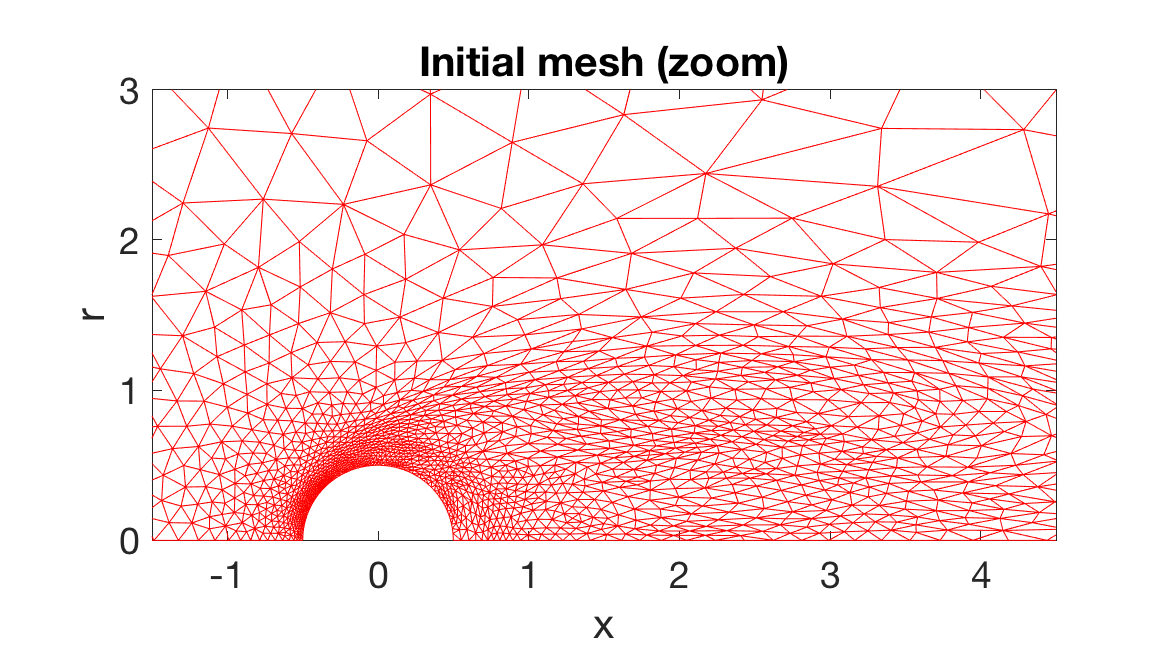
\includegraphics[width=.9 \linewidth]{Cylinder_Mesh.png}
%\vspace{-.5cm}
%\vspace{-.5cm}
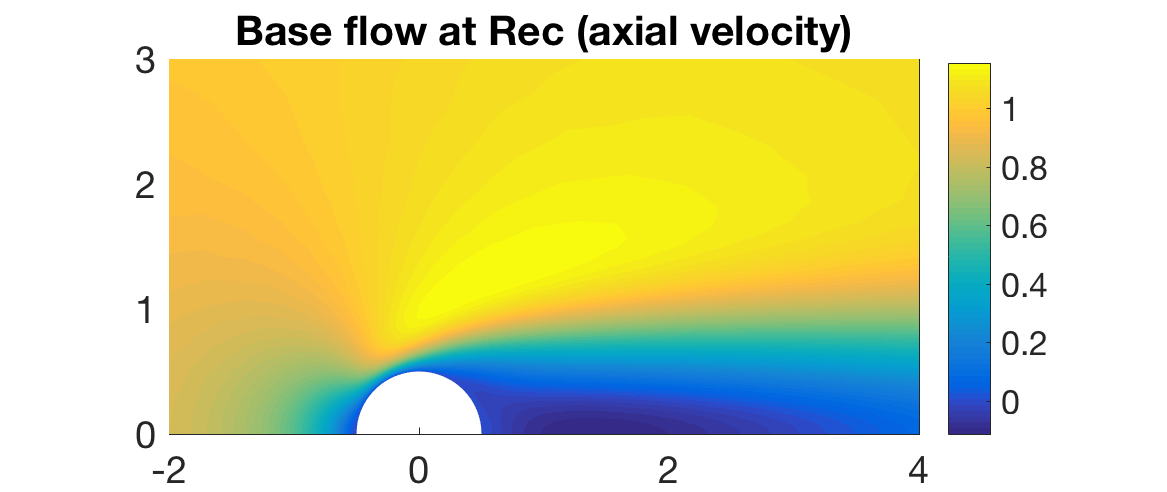
\includegraphics[width=.9 \linewidth]{Cylinder_BaseFlowReC.png}
%\vspace{-1.cm}
\caption{Adapted mesh $(a)$  and base flow (axial velocity component) ($b$) for the flow over a cylinder at $Re=Re_c = 46.7$.}
\label{fig:Baseflow}
\end{figure}

\begin{figure}
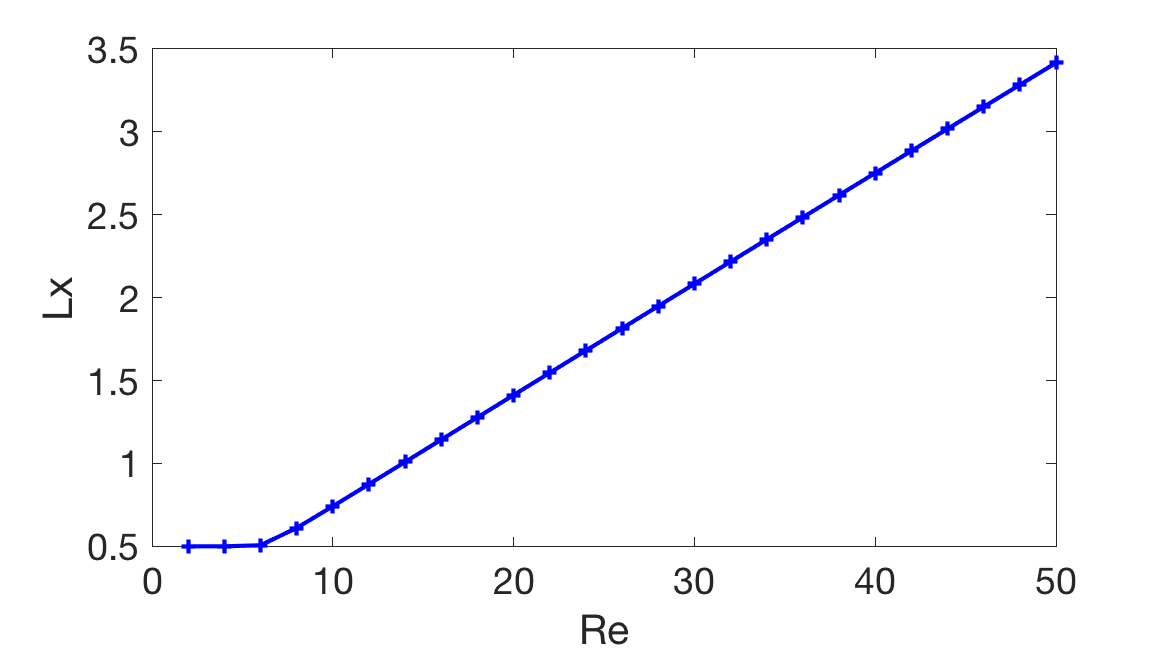
\includegraphics[width=.9 \linewidth]{Cylinder_Lx_baseflow.png}
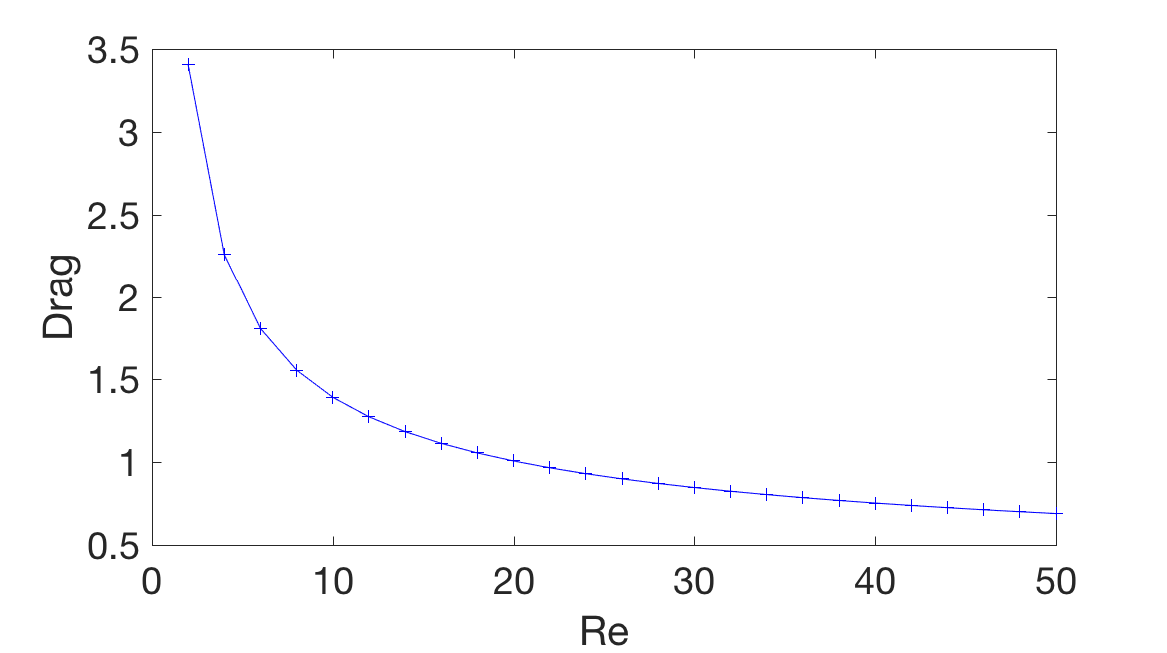
\includegraphics[width=.9 \linewidth]{Cylinder_Drag_baseflow.png}
\caption{Recirculation length $L_x$ $(a)$  and drag $C_x$ ($b$) of the base flow over a cylinder as function of $Re$.}
\label{fig:LxandDrag}
\end{figure}



\section{Illustration for the wake of a cylinder} 
\vspace{.2cm}

\paragraph{Problem description}

We will now illustrate the applicati

\paragraph{Mesh adaptation procedure}



\paragraph{Base flow}

Having thus produced an convenient mesh, we can now illustrate the properties of the base flow as function of Reynolds number. Figure (\ref{Listing2}) shows how to compute and plot with StabFem the two most commonly studied quantities, namely the drag coefficient $C_x(Re)$  and the recirculation length $Lx(Re)$, namely the location of the stagnation point at the rear of the recirculation region. 
Note that the object \verb|baseflow| is defined as a structure with fields \verb|Drag| and \verb|Lx|. 
The resulting plots are given in figure (\ref{fig:LxandDrag}), and are in good agreement with known results for this classical problem.
In particular, for low Reynolds, the recirculation $L_x(Re)$ is equal to $0.5$ (which is the radius of the cylinder) indicating the absence of a recirculation region. The latter appears for $Re > 4.8$, in accordance with known results.




%\subsection{Implementation}

%\subsection{Application to the cylinder}


%\clearpage

%We now review the main concepts of linear stability approach and explain how such calculations are implemented in our software.


\begin{figure}
%\vspace{-.5cm}
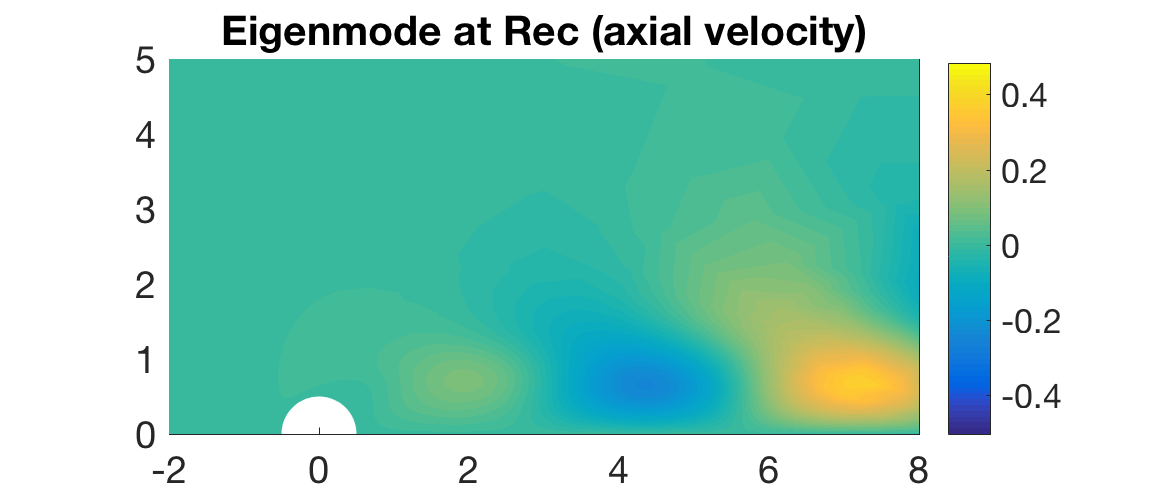
\includegraphics[width=.9 \linewidth]{Cylinder_EigenModeReC.png}
%\vspace{-.5cm}
%\vspace{-.5cm}
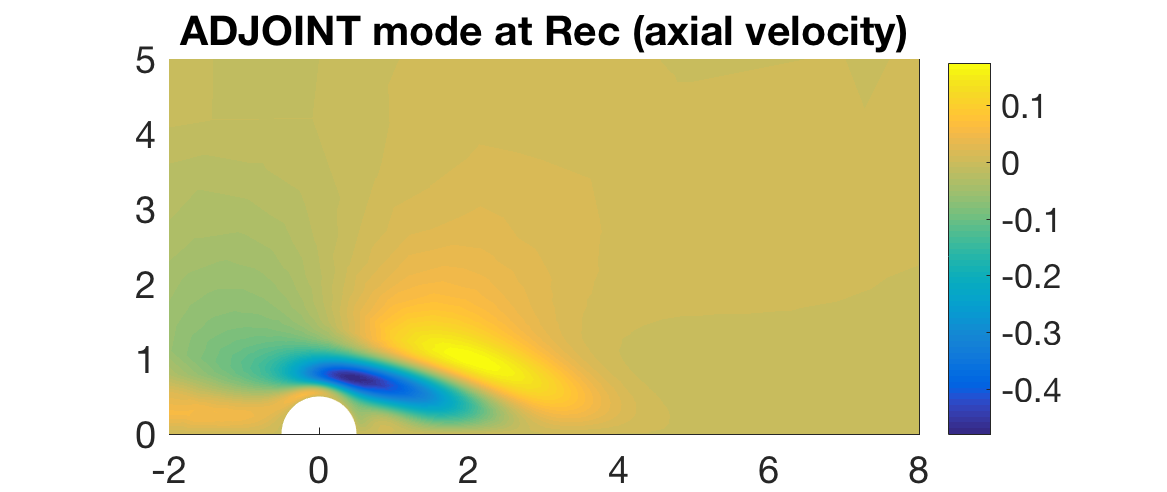
\includegraphics[width=.9 \linewidth]{Cylinder_EigenModeAdjReC.png}
%\vspace{-.5cm}\vspace{-.5cm}
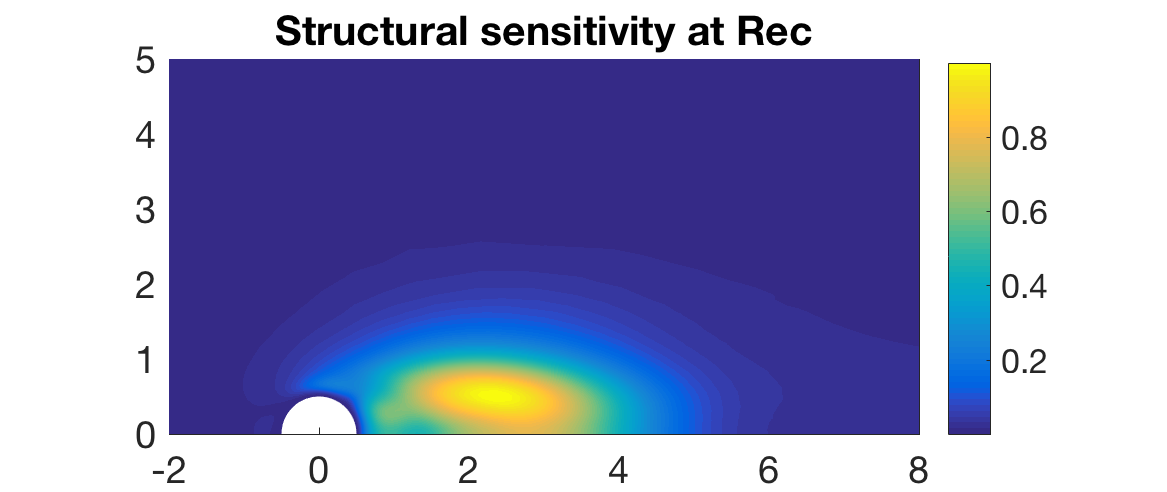
\includegraphics[width=.9 \linewidth]{Cylinder_SensitivityReC.png}
%\vspace{-.5cm}
\caption{Eigenmode $(a)$  (axial velocity component),  Adjoint mode $(b)$ and structural sensitivity ($c$) for the cylinder's wake at $Re=Re_c = 46.7$.}
\label{fig:Eigenmode}
\end{figure}


\begin{figure}
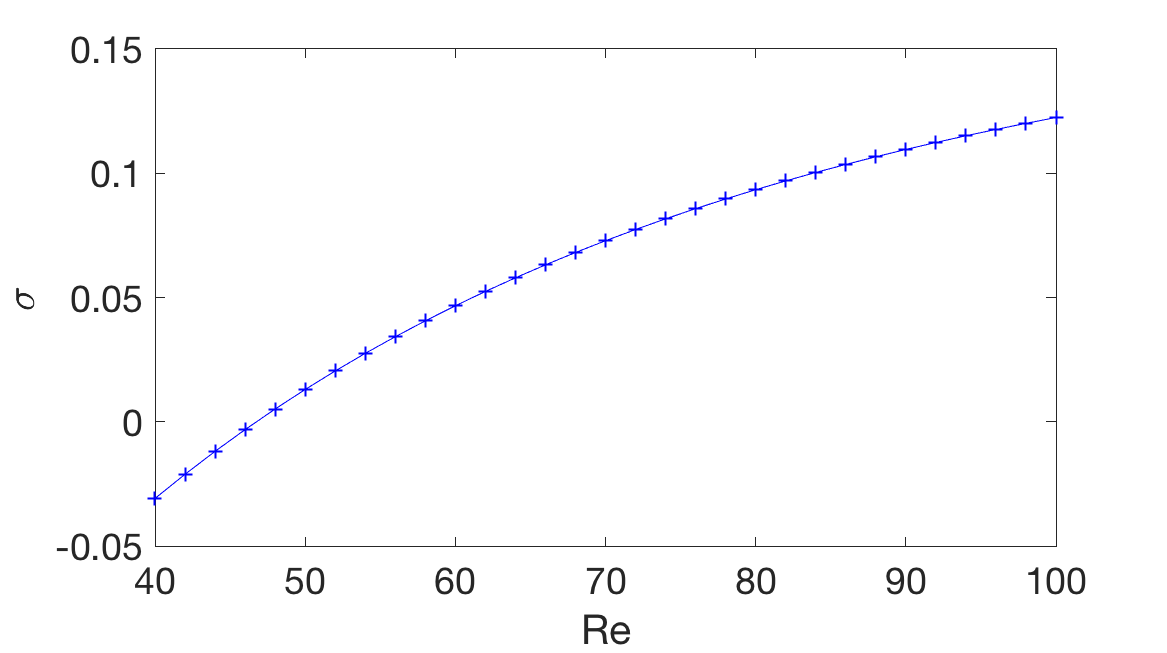
\includegraphics[width=.9 \linewidth]{Cylinder_Sigma_Re.png}
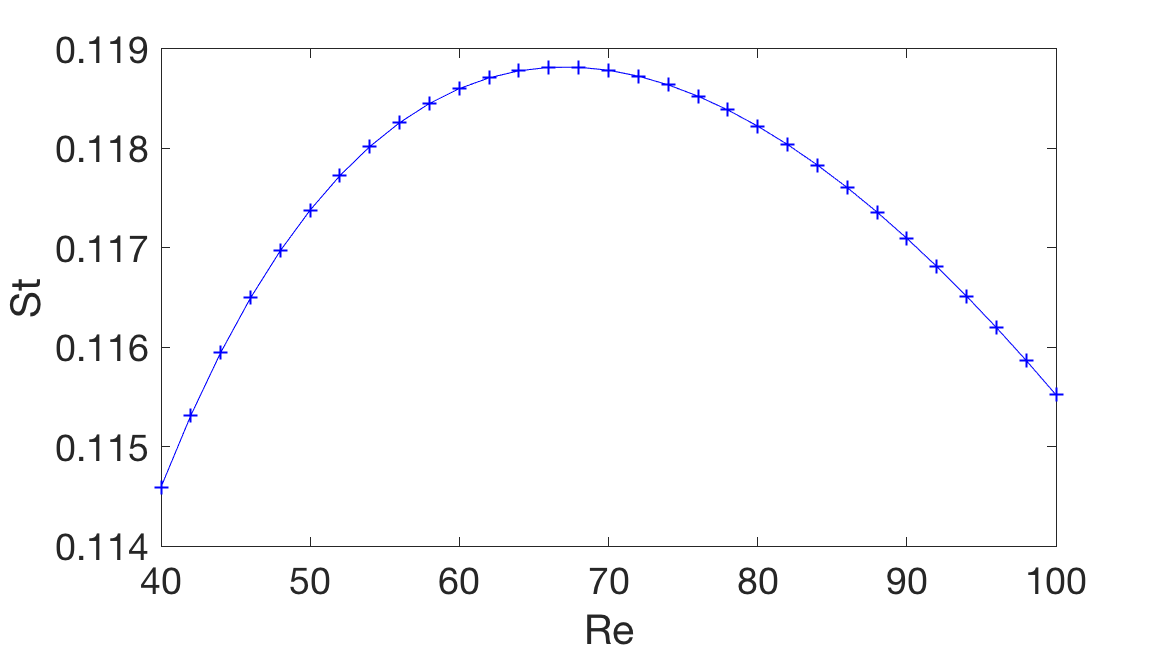
\includegraphics[width=.9 \linewidth]{Cylinder_Strouhal_Re.png}
\caption{Growth rate $\sigma$ $(a)$  and Strouhal number $St = (a \omega)/(2\pi U_0)$ ($b$) as function of Reynolds number}
\label{fig:SigmaOmega}
\end{figure}

%\begin{figure*}
%\small
%\begin{lstlisting}
%\end{lstlisting}
%\normalsize
%\caption{Illustration of the procedure to compute stability properties and adapt the mesh using StabFem (from script {\em SCRIPT\_CYLINDER.m}. }
%\label{listing4}
%\end{figure*}

\paragraph{Linear stability results}


 
%popular class of method are {\em power methods} which allow to compute a limited set 

%based on the idea that the repeated application of an operator mostly amplifies the perturbations along the eigenspaces with largest eigenvalues. 

%These de Andrea Fani



%\paragraph{Implementation and mesh adaptation for stability calculations}



Matlab driver...


%\paragraph{Sample results}



%\subsection{Illustration of the mesh adaptation for stability calculations}

%See listing....

%\subsection{Sample results for a cylinder}

%\clearpage

\section{Nonlinear global stability approaches}
\vspace{.2cm}
%\section{Computing the limit cycle for $Re>Re_c$ with Harmonic Balance}

\paragraph{Review on nonlinear global stability approaches}
%For $Re\right>Re_c$, the linear stability analysis based on the {\em base flow} does not allow to predict the properties of the limit cycle; in particular the Strouhal number is substantially underestimated. %It has been shown that investigating the stability properties of the {\em mean flow} obtained by averaging time-marching solution gives a better accordance. Attempts to on a rigourous basis  
In the past decade, efforts have been devoted to extend the range of validity of global approaches into the nonlinear régime for $Re>Re_c$, with the double objective to describe the properties of the limit cycle reached after saturation and to derive amplitude equations describing the transitent dynamics towards this cycle.
 The first milestone in that direction is the work of Sipp \& Lebedev who used a weakly nonlinear development in terms of the distance to the threshold $Re-Re_c$. However, although derived on rigorous grounds, the weakly nonlinear development has a very limited range of validity and already fails for $Re\ge47$.
More recently,  Mantic-lugo et al.  proposed an alternative approach termed {\em Self-consistent model} which succeeds in predicting the dynamics up to $Re =120$ and more. 
This model was build as a linear stability approach build on a {\em mean flow} which includes a 
retroaction of the eigenmode. However, if one is interested in the limit cycle and not the transient,
the approach is actually equivalent to a Fourier series decomposition of the flow with respect to time (an approach also known as {\em harmonic balance}) retaining only the two first terms. 
%The approach is based on a generalisation of the eigenmode ansatz \ref{} and 

In the next section we thus present this model and propose a direct resolution method. The relation with the initial method of Mantic-Lugo et al. will be discussed afterwards.

\paragraph{Harmonic balance : equations and procedure }

In this section, to simplify the notations, The Navier-Stokes equations will be written symbolically as 
$\partial_t  {\bf u }  = NS(  {\bf u } )$, therefore droping the systematic reference of the incompressibility constraint and associated pressure field.

We thus start with a Fourier decomposition of the limit cycle under the form :
\be{HB}
{\bf u } = {\bf u }_0 + {\bf u }_1 e^{i \omega t} +   {\bf u }_{-1} e^{-i \omega t}
\ee  
Here ${\bf u }_0$ is the mean flow (averaged over time),  ${\bf u }_1$ is the mode
(fourrier component at the fundamental frequency), ${\bf u }_{-1} = \overline{{\bf u }_1}$ is its complex conjugate, and $\omega$ is the (real) oscillation frequency of the limit cycle (which is not known a priori). Injecting this ansartz into the Navier-Stokes equations and taking the mean value and first Fourier component leads to the following coupled equations :
\be{HBEq0}
NS(  {\bf u }_0 ) - {\cal C}( {\bf u }_1, \overline{\bf u }_1) = 0,
\ee
\be{HBEq1}
i \omega {\bf u }_1 =  NSL_{{\bf u }_0}(  {\bf u }_1 ).
\ee

Note that the Fourier description of the limit cycle is invariant with respect to the phase $\phi$ (i.e. the equations are unchanged when replacing $[ {\bf u }_1,  {\bf u }_{-1}] $ by  $[ {\bf u }_1 e^{i\varphi},  {\bf u }_{-1}  e^{-i\varphi}] $. 
To allow resolution we thus need an extra equation to fix this phase. Several choices are possible, but a convenient one is to set the lift associated with the imaginary part of ${\bf u }_1$ to lift. Physically, this means that the instant $t=0$ will correspond to a maximum of lift. This condition reads :
\be{HBphase}
\Im F_y({\bf u}_1) =0
\ee

With $F_y ({\bf u_1}) = 
 \int_{\Gamma_w} \left[-p_1 {\bf n} + \frac{2}{Re} {\bf D}({\bf u_1}) \cdot {\bf n} \right]   \cdot {\bf e_y}  = 0.$


Mathematically, the problem $\ref{HBEq0,HBEq1,HBphase}$ for the unknown $[{\bf u }_0, {\bf u }_{1}, \omega]$ is well posed, and can be solved using a Newton iteration just as explained for the base flow in section 2. To allow resolution, we separate the mode into real and imaginary part, by writing ${\bf u }_1 = {\bf u }_{1,r} +  i {\bf u }_{1,i} $.
We then assume that we know a 'guess' 
$$
[{\bf u }_0, {\bf u }_{1,r}, {\bf u }_{1,i}, \omega] = 
 [{\bf u }_0^g, {\bf u }_{1,r}^g, {\bf u }_{1,i}^g, \omega^g]
+ [\delta {\bf u }_0, \delta {\bf u }_{1,r}, \delta {\bf u }_{1,i}, \delta \omega]
$$.

Injecting and developing up to linear order leads to the following 
\begin{equation}
\begin{array}{ll}
\displaystyle
& NS(  {\bf u }_0^g ) - [ {\cal C}( {\bf u }_{1,r}^g,{\bf u }_{1,r}^g) +  {\cal C}( {\bf u }_{1,i}^g,{\bf u }_{1,i}^g) ]
\\
+& NSL_{{\bf u }_0^g}(\delta {\bf u }_0) - 2 [ {\cal C}( {\bf u }_{1,r}^g,\delta {\bf u }_{1,r}) +  {\cal C}( {\bf u }_{1,i}^g,\delta {\bf u }_{1,i}) ] = 0;
\\
\\
&  NSL_{{\bf u }_0^g}( {\bf u }_{1,r}^g) - \omega^g {\bf u }_{1,i}^g 
 \\
  +& NSL_{{\bf u }_0^g}( \delta {\bf u }_{1,r}^g) 
   -  {\cal C}( \delta {\bf u }_{0}^g, {\bf u }_{1,r})
   - \delta \omega^g \delta {\bf u }_{1,i}^g 
 - \omega^g \delta {\bf u }_{1,r} = 0 ;
 \\
\\
&  NSL_{{\bf u }_0^g}({\bf u }_{1,i}^g) + \omega^g {\bf u }_{1,i}^g
 \\
  +& NSL_{{\bf u }_0^g}( \delta {\bf u }_{1,i}^g) 
  -  {\cal C}( \delta {\bf u }_{0}^g, {\bf u }_{1,i}) 
  + \delta \omega^g \delta {\bf u }_{1,i}^g 
+ \omega^g \delta {\bf u }_{1,r} = 0 ;
\\
\\
& F_y({\bf u }_{1,i}^g) + F_y(\delta {\bf u }_{1,i}) = 0.
 \end{array}
\end{equation}

After discretization, this leads to a linear problem with the form $A X = Y$ where $X$ is the discretized version of the unknowns  $[\delta {\bf u }_0, \delta {\bf u }_{1,r}, \delta {\bf u }_{1,i}, \delta \omega]$, and $A$ is a matrix of dimension $3 N_{dof} +1$. 
 
%\ref{HBEq0,HBEq1,HBphase}


\paragraph{Results for the wake of a cylinder}


\paragraph{Link with the Self-Consistent approach}

We now discuss the link between the harmonic balance approach presented above and the self-consistent approach as introduced by Mantic-Lugo et al.
The starting point of this model is a pseudo-eigenmode expansion of the flow as follows :

\be{SC}
{\bf u } = {\bf u }_m + A \left[ \tilde{{\bf u }}_1 e^{\sigma_{SC} t + i \omega_{SC} t} +   \tilde{\bf u }_{-1} e^{\sigma_{SC} t  -i \omega_{SC} t} \right]
\ee  
Where ${\bf u }_m$ is a {\em mean flow} defined by phase-averaging over the cycle, $\tilde{{\bf u }}_1$ is a pseudo-eigenvector which is normalized by the condition  $||\tilde{{\bf u }}_1|| = 1/\sqrt{2}$, 
 $A$ is an amplitude parameter directly related to the energy of the oscillating flow, and $\lambda = \sigma_{SC} + i \omega_{SC}$ is a pseudo-eigenvalue which depends upon the parameter $A$. The mean flow is then governed by the same equation
(\ref{HBEq0}) written above, while $\tilde{{\bf u }}_1$ is the solution of an eigenvalue problem with the same form as  (\ref{HBEq1}) except that $i \omega$ is replaced by $\sigma_{SC} + i \omega_{SC}$.
The self-consistent model has the following properties :
\begin{itemize}
\item[-] For $A \ll 1$ it is equivalent to the linear eigenvalue problem (\ref{LEP}), and the generalized eigenvalue coincides with the one predicted by linear stability : $\sigma_{SC} + i \omega_{SC} = \sigma_{lin} + i \omega_{lin}$. 
\item[-] For $\sigma_{SC}=0$ (corresponding to a specific choice of the amplitude $A=A_c$),  the expansion (\ref{SC}) is equivalent to the harmonic-balance decomposition (\ref{HB})
\item[-] For $0<A<A_c$, the resolution leads to a relation $\sigma_{SC}(A) ; \omega_{SC}(A)$
such that $0< \sigma_{SC}(A) < \sigma_{lin}$.
 Although in this case the expansion \ref{SC} cannot represent the flow for all $t$, Mantic-Lugo et al. argued that the relation between $\sigma_{SC}$ and $A$ can be used to build an amplitude equation which captures the transient approach to the limit cycle. 
\end{itemize}




%Barkley [] and Leontini [] have 




\begin{figure}
\begin{center}
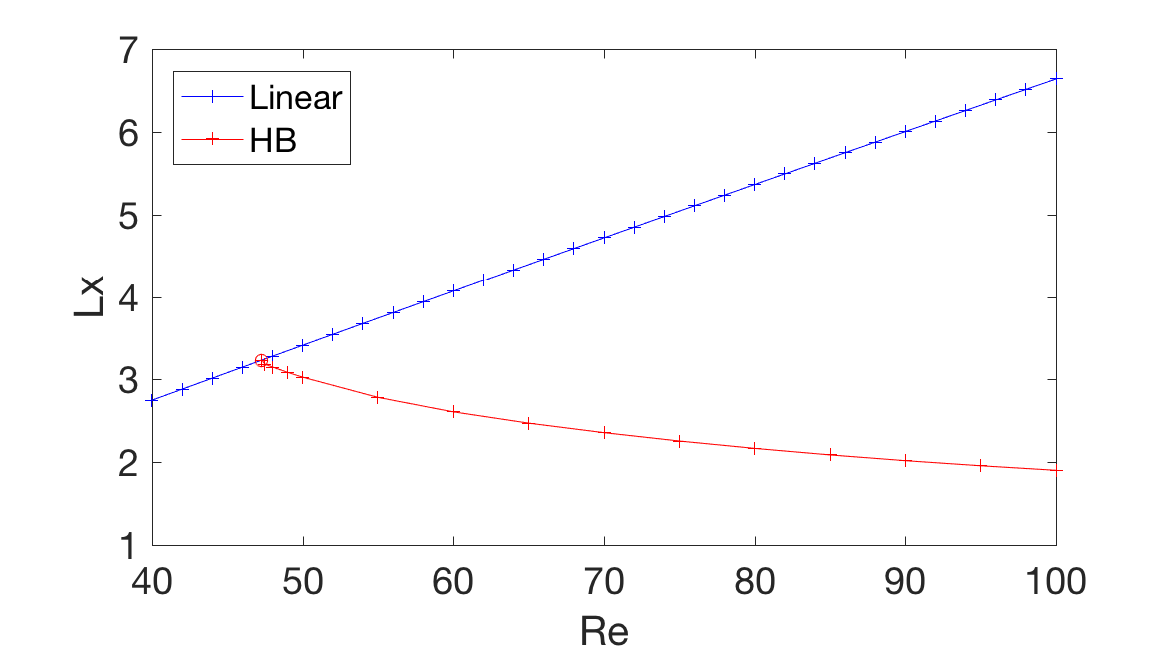
\includegraphics[width=.9 \linewidth]{Cylinder_Lx_Re_HB.png}
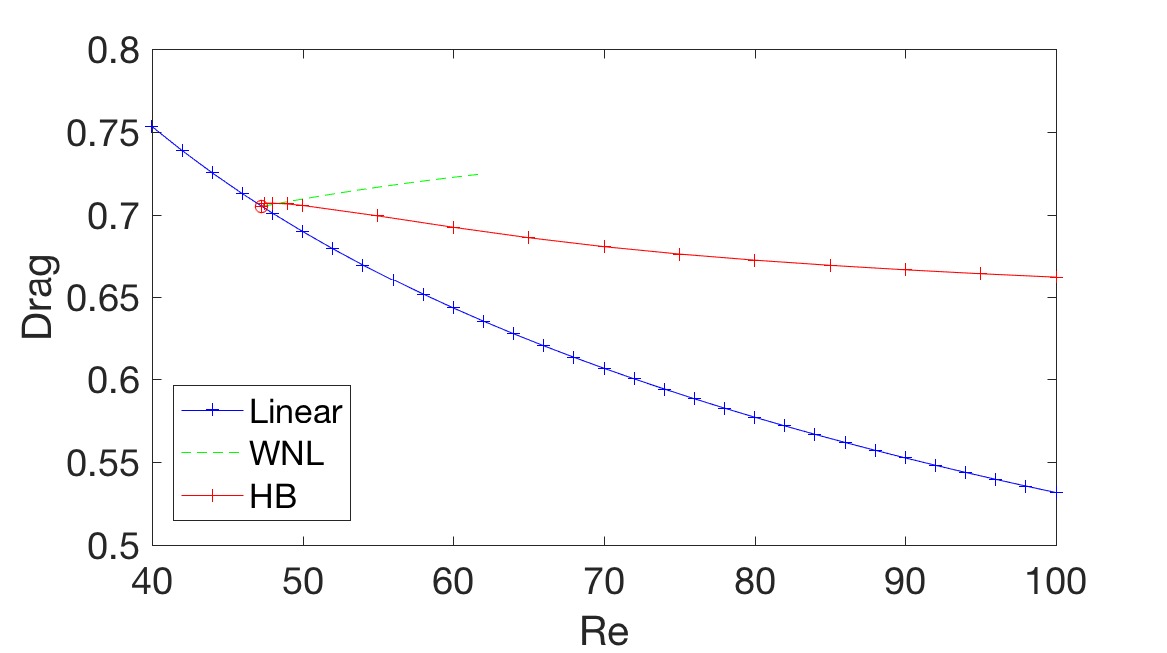
\includegraphics[width=.9 \linewidth]{Cylinder_Drag_Re_HB.png}
\end{center}
\caption{Harmonic-balance results : mean-flow characteristics}
\label{fig:HB}
\end{figure}

\begin{figure}
\begin{center}
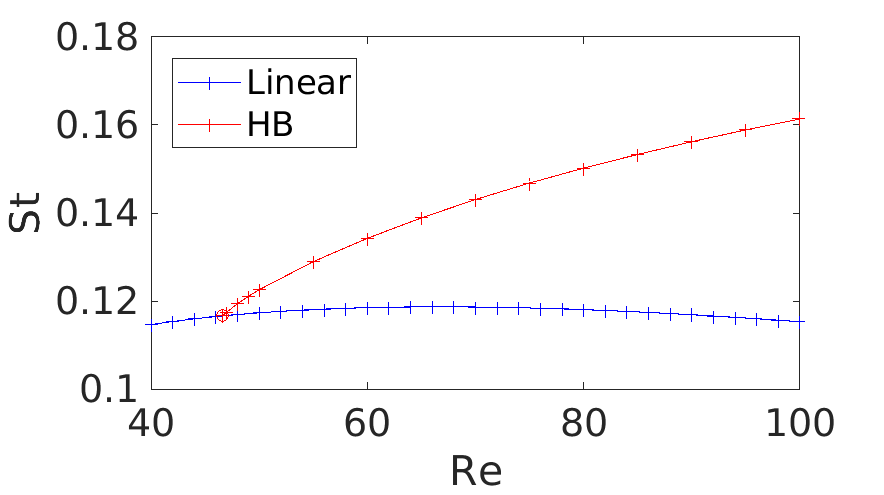
\includegraphics[width=.9 \linewidth]{Cylinder_Strouhal_Re_HB.png}
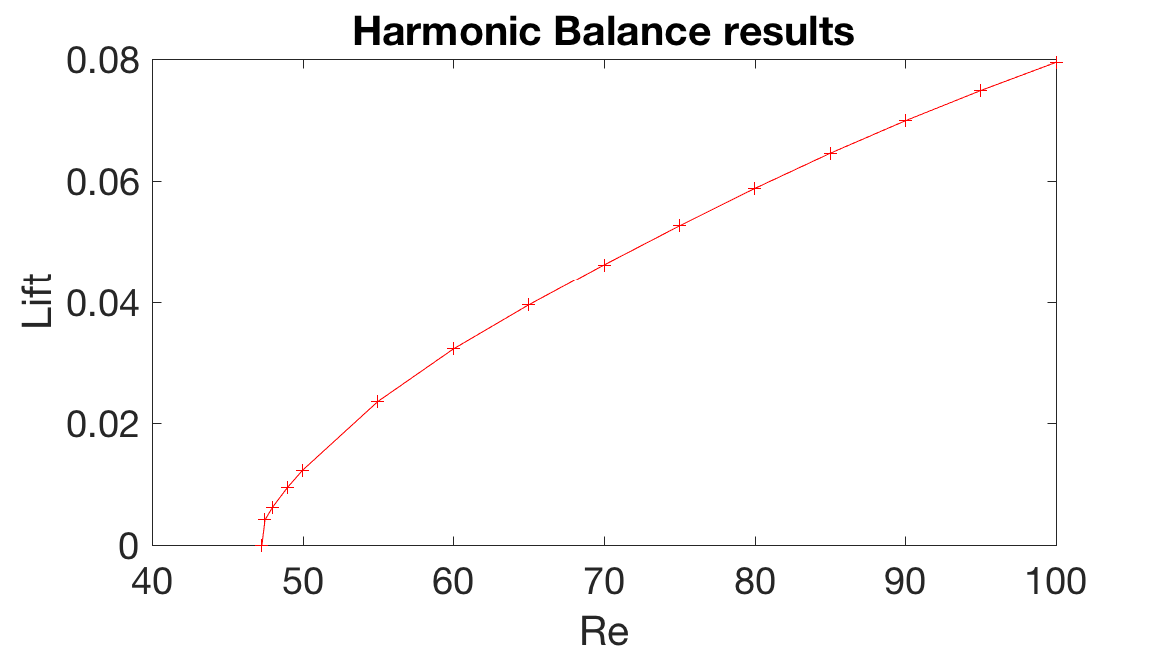
\includegraphics[width=.9 \linewidth]{Cylinder_Lift_Re_SC.png}
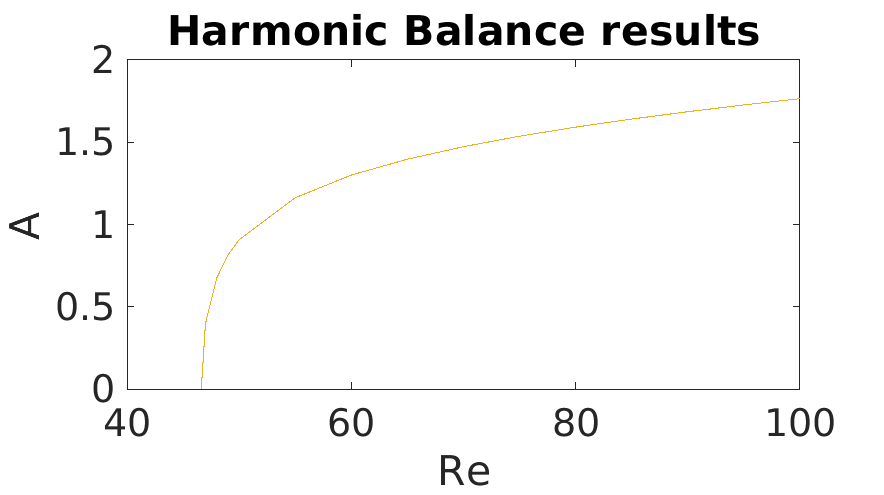
\includegraphics[width=.9 \linewidth]{Cylinder_Energy_Re_SC.png}
\end{center}
\caption{Harmonic-balance results : mode characteristics}
\label{fig:HB}
\end{figure}

\begin{figure}
\begin{center}
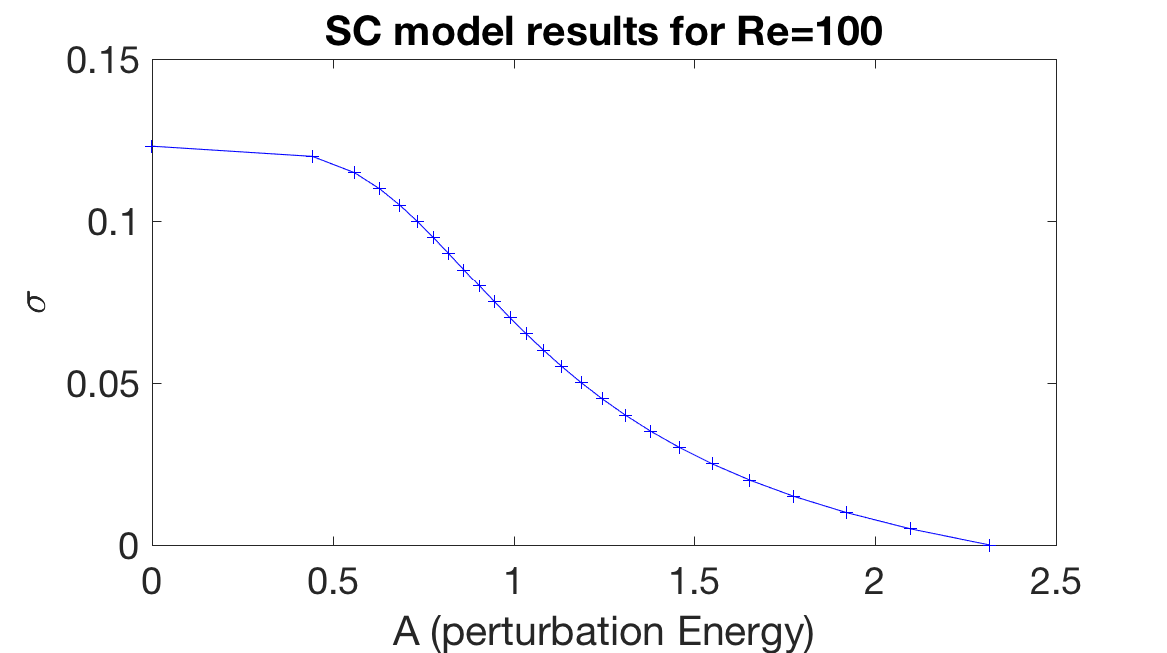
\includegraphics[width=.9 \linewidth]{Cylinder_SC100_EnergySigma.png}
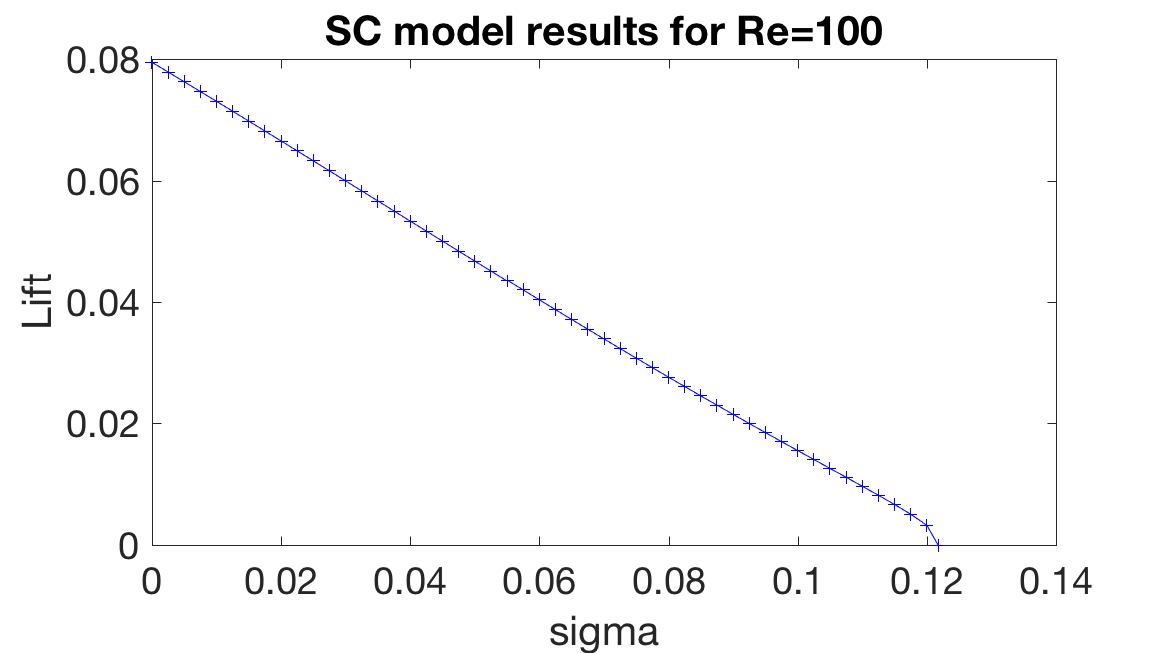
\includegraphics[width=.9 \linewidth]{Cylinder_SC100_LiftSigma.png}
\end{center}
\caption{SELF CONSISTENT APPROACH FOR THE WAKE OF A CYLINDER, $Re = 60$}
\label{fig:SC60}
\end{figure}






\appendix

\section{Appendix : details on mesh convergence}


\paragraph{Illustration of mesh convergence procedure for a cylinder}

\begin{figure*}
\small
\begin{lstlisting}
> baseflow=SF_Init('Mesh_Cylinder_Large.edp');
      ### INITIAL MESH CREATED WITH np = 2207 points
> baseflow=SF_BaseFlow(baseflow,'Re',1);
      ### FUNCTION SF_BaseFlow : computing base flow for Re = 1
      # Base flow converged in 6 iterations ; Drag = 5.9876; Lx = 0.501
> baseflow=SF_BaseFlow(baseflow,'Re',10);
      ### FUNCTION SF_BaseFlow : computing base flow for Re = 10
      # Base flow f converged in 5 iterations ; Drag = 1.4519; Lx = 0.73191
> baseflow=SF_BaseFlow(baseflow,'Re',60);
      ### FUNCTION SF_BaseFlow : computing base flow for Re = 60
      # Base flow converged in 6 iterations ; Drag = 0.66348; Lx = 3.6989

> baseflow=SF_Adapt(baseflow,'Hmax',10,'InterpError',0.01);
     ### ADAPT mesh to base flow ; InterpError = 0.01  ; Hmax = 10
      #   Number of points np = 1352 ; Ndof = 11862
      #  h_min, h_max : 0.018824 , 10.2895
      #  h_(A,B,C,D) : 0.027467 , 0.28644 , 0.45948 , 0.89245
      ### FUNCTION SF_BaseFlow : computing base flow for Re = 60
      # Base flow converged in 5 iterations ; Drag = 0.65805; Lx = 4.0737

> plotFF(baseflow,'mesh');



\end{lstlisting}
\normalsize

\caption{Illustration of the procedure to compute a base flow and an adapted mesh using StabFem (from script {\em SCRIPT\_CYLINDER.m}. }
\end{figure*}

\begin{figure*}
\small
\begin{lstlisting}
> [ev,em] = SF_Stability(baseflow,'shift',0.04+0.76i,'nev',1,'type','D');
> [baseflow,em]=SF_Adapt(baseflow,em,'Hmax',10,'InterpError',0.005);  
      ### ADAPT mesh to base flow AND MODE   ; InterpError = 0.005  ; Hmax = 10
      #   Number of points np = 13458 ; Ndof = 120030
      #  deltamin, deltapax : 0.0089891 , 13.367
      #  delta_(A,B,C,D) : 0.020536 , 0.082852 , 0.07316 , 0.11914
      ### FUNCTION SF_BaseFlow : computing base flow for Re = 60
      # Base flow converged in 4 iterations ; Drag = 0.64695; Lx = 4.0715
      ### FUNCTION SF_Stability : computation of 1 eigenvalues/modes (DIRECT) with FF solver
      # Stability calculation converged in 4 iterations, lambda = 0.047152+0.74808i.

> [ev,em] = SF_Stability(baseflow,'shift',0.04+0.76i,'nev',1,'type','S');
> [baseflow,em]=SF_Adapt(baseflow,em,'Hmax',10,'InterpError',0.005);
      ### ADAPT mesh to base flow AND SENSITIVITY ; InterpError = 0.005  ; Hmax = 10
      #   Number of points np = 4355 ; Ndof = 38559
      #  deltamin, deltapax : 0.0058536 , 13.1164
      #  delta_(A,B,C,D) : 0.01049 , 0.091861 , 0.13319 , 0.89372
      ### FUNCTION SF_BaseFlow : computing base flow for Re = 60
      # Base flow converged in 3 iterations ; Drag = 0.64758; Lx = 4.0725
      ### FUNCTION SF_Stability : computation of 1 eigenvalues/modes (DIRECT) with FF solver
      # Stability calculation converged in 3 iterations (D+A+S), lambda = 0.047165+0.74823i.

\end{lstlisting}
\normalsize

\caption{Illustration of the procedure to adapt the mesh for stability calculations with StabFem (from script {\em SCRIPT\_CYLINDER.m}. }
\end{figure*}



We illustrate the procedure in the case of a cylinder.  Figure 1 gives a retranscription of the sequence of commands (from {\em SCRIPT\_CYLINDER\_ADAPTMESH\_BASEFLOW}) 
and the output produced.
First we build an initial mesh (line 1), and compute base flow solutions for increasing values of the Reynolds number up to $Re = 60$ (lines 3-9).

Then we perform the mesh adaptation (line 13). The produced outputs (lines 14-17) gives information about the resulting mesh. 
Note the values $h_{min}$ and $h_{max}$ of the smaller and larger edges, as well as the local grid size at four points A,B,C,D defined as $(x_A,y_A) = (0.5,0)$ (at the surface of the cylinder at the position of maximum shear), $(x_B,y_B) = (0.5,2.5)$ (at the location of the peak of structural sensitivity, see next section), $(x_C,y_C) = (0.,4)$ (in the near wake), and $(x_D,y_D) = (0.,10)$ (in the the far wake). Finally, the base flow is automatically recomputed on the resulting mesh (line 18-19). Finally, lines 21-22 plot the mesh and base flow structure, producing the result displayed in figure (\ref{fig:Baseflow}).



\begin{figure*}
\small
\begin{lstlisting}
\end{lstlisting}
\normalsize

\caption{Illustration of the procedure to adapt the mesh for stability calculations with StabFem (from script {\em SCRIPT\_CYLINDER.m}. }
\label{listing3}
\end{figure*}


\section{Detail of the weak formulation}
%The problem can be set into weak form by multiplying by multiplying Eq. \ref{Newton2} by a test function ${\bf v}$ and the associated divergence constraint by a test function $q$. After a few integration by parts we are led to :
\begin{eqnarray}
\label{NewtonWeak}
&\forall ({\bf v};q), \\
\displaystyle &\int \left[ {\bf v} \cdot {\cal C}( {\bf u}_b^g , \delta {\bf u}_b) +  \nabla  \cdot \delta {\bf u}_b q -\nabla  \cdot {\bf v} \delta p_b
+ \frac{2}{Re} {\bf D}(\delta {\bf u}_b) : {\bf D}({\bf v}) \right]
\nonumber
\\
\nonumber
\displaystyle & + \int \left[ {\bf v} \cdot ( {\bf u}_b^g \cdot \nabla {\bf u}_b^g) 
+ \nabla \cdot {\bf u}_b^g  q 
- \nabla \cdot {\bf v} p_b^g
+ \frac{2}{Re} {\bf D}({\bf u}_b^g) : {\bf D}({\bf v}) \right] = 0 
\end{eqnarray}


\end{document}


 